% !TEX root = lie-groups.tex
\section{Lie Groups}

Historically and in practice, Lie groups arise first as the study of the transformation of geometric objects.
Let us consider the example of a sphere in euclidean space.
There are in a sense three ways to rotate a sphere.
Choose a point on the equator of a sphere.
You can rotate the sphere so that this point moves towards a pole (y-axis rotation), so that this point moves along the equator (z-axis rotation), or so that the point is stationary (x-axis rotation).
Moreover these rotations are continuous in a way that rotating an equilateral triangle is not, because at each stage of rotation the sphere as a whole occupies the same space.

How should we describe the rotations of a sphere?
First observe that antipodal points remain antipodal, so the rotation of a sphere extends to a linear transformation of $\bbR^3$.
Hence any rotation $R$ can be described by a real $3\times 3$-matrix.
Moreover rotation is length and angle preserving, so $\langle Rx, Ry \rangle = \langle x, y \rangle$.
This holds exactly if $R^TR = I$, which gives us the orthogonal group
\[
\lgO(3) = \{ R \in \Mat(3,\bbR) \mid R^TR = I \}.
\]
We can understand the defining equation as saying that the columns of $R$ are an orthonormal basis of $\bbR^3$.
Indeed they are the images of the standard basis of $\bbR^3$ under $R$.
By rotations we mean proper rotations, which are by definition orientation preserving, so we want that the columns of $R$ are a right handed basis.
That leads to the special orthogonal group
\[
\lgSO(3) = \{ R \in \lgO(3) \mid \det R = 1 \}.
\]
The group operation is composition of operators, ie matrix multiplication.
Both groups clearly contain the identity $I$.
The property $R^T R = I$ implies $(\det R)^2 = 1$, so these are invertible matrices.
Therefore they really are groups.
Moreover the sign of the determinant can be used to distinguish a proper rotation from an improper one.
% The later group are the (proper) rotations, the former is a group that includes reflections.

Heuristically, we have nine choices for the matrix of $R$ subject to the restriction each of the three columns must be unit length and the restriction that pairs of columns must be orthogonal (six restrictions total).
This agrees with the three degrees of freedom we argued for above.
To see this is a manifold however we consider a function $f$ from $\Mat(3,\bbR)$ to the symmetric matrices given by $f(R) = R^TR$.
The orthogonal matrices are exactly $\lgO(3) = f^{-1}(I)$.
The derivative at $R$ in the direction $S$ is $f'(R)(S) = R^TS + S^T R = R^T S + (R^T S)^T$.
At a point $R \in \lgO(3)$ this is surjective in $S$: for any symmetric matrix $Y$ let $S = \frac{1}{2}RY$.
Hence $f$ is full rank at every point $R \in \lgO(3)$ and by the implicit function theorem $\lgO(3)$ is an embedded submanifold of $\Mat(3,\bbR) \cong \bbR^9$.
The symmetric matrices are dimension $6$, so in fact our heuristic has been formalised to a rigorous argument.

The group operation, matrix multiplication, is a smooth operation on the set of matrices because it is polynomial.
Therefore it is also smooth when restricted to an embedded submanifold.
Similarly inversion is an everywhere defined rational function on the open set of invertible matrices, so also smooth on $\lgO(3)$.
This makes $\lgO(3)$ and $\lgSO(3)$ Lie groups.

Now that we know that $\lgO(3)$ is a manifold, we can ask about its connected components.
Intuitively we can rotate any right handed frame $R \in \lgSO(3)$ to the standard basis $I$, so $\lgSO(3)$ is connected.
Because it contains the identity, it is called the identity component.
On the other hand, the reflection in the plane $x_1 = 0$ has determinant $-1$ whereas $\det I = 1$.
Determinant is continuous (polynomial) function on matrices and as already noted $R \in \lgO(3)$ implies $\det R = \pm 1$, so this reflection is not in the identity component.
Composing an improper rotation with this reflection gives a proper rotation and vice-versa. Therefore the subset of $\lgO(3)$ with $\det R = -1$ is also a connected component of $\lgO(3)$.
In conclusion, $\lgSO(3)$ is connected and $\lgO(3)$ has two diffeomorphic components.

To understand the topology of $\lgSO(3)$ an alternate description is useful.
Every rotation of $\bbR^3$ is rotation around an axis.
More precisely, we can describe the rotation axis by a unit vector $u$ such that the rotation is right handed by an angle $\theta$ in the range $[0,\pi]$.
Thus the rotations can be described by the closed unit ball $\theta u \in \overline{B(0,1)}$.
The origin is rotation by angle $0$ with the axis of rotation irrelevant.
But similarly, rotation by $\pi$ around $u$ and $-u$ are the same rotation.
Thus $\lgSO(3)$ can be modelled as the closed unit ball with antipodal points on the boundary identified, the real projective space $\RP^3$.

In this model it is easy to understand the fundamental group.
Take any closed loop in $\lgSO(3)$.
If it lies entirely in $B(0,1)$ then it can be contracted to a point.
% If it meets $\partial B(0,1)$ in one point then we may describe it as a path $\gamma : (0,1) \to B(0,1)$ with $\gamma(1) = - \gamma(0) \in \partial B(0,1)$. 
Otherwise it can be divided into a collection of segments $\gamma_i : (0,1) \to B(0,1)$ with $\gamma_{i+1}(0) = \pm \gamma_i(1) \in \partial B(0,1)$ and $\gamma_1(0) = \pm \gamma_n(1) \in \partial B(0,1)$.
These conditions ensure that the segments connect up to a loop in $\RP^3$.
We call the number of negative signs the index of the loop.
If $\gamma_{i+1}(0) = \gamma_i(1)$ then it is possible to move this point into the interior of $B(0,1)$ and fuse these two segments together into a single segment.
This doesn't change the index of the loop.
As an extreme case, if the index is zero, then we can move all the endpoints of the segments off $\partial B(0,1)$ and contract the loop to a point.
So without loss of generality, assume that all the signs are negatives.
\begin{center}
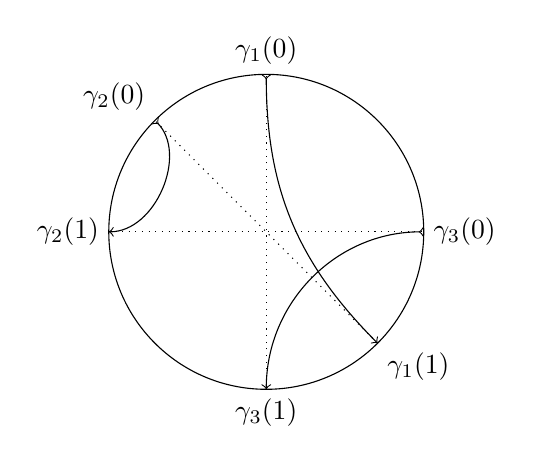
\begin{tikzpicture}
    % Circle
    \draw (0,0) circle (2cm);
    
    % Curve 1
    \draw[>->] (90:2cm) to[out=270, in=135] (-45:2cm);
    \node at (90:2cm) [above] {$\gamma_1(0)$};
    \node at (-45:2cm) [below right] {$\gamma_1(1)$};

    \draw[dotted] (-45:2cm) -- (135:2cm);
    
    % Curve 2
    \draw[>->] (135:2cm) to[out=-45, in=0] (180:2cm);
    \node at (135:2cm) [above left] {$\gamma_2(0)$};
    \node at (180:2cm) [left] {$\gamma_2(1)$};

    \draw[dotted] (180:2cm) -- (0:2cm);

    % Curve 3
    \draw[>->] (0:2cm) to[out=180, in=90] (-90:2cm);
    \node at (0:2cm) [right] {$\gamma_3(0)$};
    \node at (-90:2cm) [below] {$\gamma_3(1)$};

    \draw[dotted] (-90:2cm) -- (90:2cm);
\end{tikzpicture}
\begin{tikzpicture}
    % Circle
    \draw (0,0) circle (2cm);
    
    % Curve 1
    \draw[>->] (90:2cm) to[out=270, in=110] (0:2cm);
    \node at (90:2cm) [above] {$\gamma_1(0)$};
    % \node at (-45:2cm) [below right] {$\gamma_1(1)$};

    % \draw[dotted] (-45:2cm) -- (135:2cm);
    
    % Curve 2
    \draw[>->] (180:2cm) to[out=45, in=180] (150:1.5cm) to[out=0, in=0]  (180:2cm);
    % \node at (135:2cm) [above left] {$\gamma_2(0)$};
    \node at (180:2cm) [left] {$\gamma_2(0) = \gamma_2(1)$};

    \draw[dotted] (180:2cm) -- (0:2cm);

    % Curve 3
    \draw[>->] (0:2cm) to[out=180, in=90] (-90:2cm);
    \node at (0:2cm) [right] {$\gamma_1(1)=\gamma_3(0)$};
    \node at (-90:2cm) [below] {$\gamma_3(1)$};

    \draw[dotted] (-90:2cm) -- (90:2cm);
\end{tikzpicture}
\end{center}
If there is more than one segment, we can move $\gamma_1$ and $\gamma_2$ such that $\gamma_1(0)$ and $\gamma_2(1)$ remain fixed (so no other segments are affected) but $\gamma_2(0)$ is moved to $\gamma_2(1)$ (so necessarily $\gamma_1(1) \to - \gamma_2(1)$).
Then $\gamma_2$ can be contracted to the constant map $\gamma_1(1) = -\gamma_2(0) = -\gamma_2(1) = \gamma_3(0)$.
This means that we can eliminate $\gamma_2$ and fuse $\gamma_1$ and $\gamma_3$ into a single segment.
In particular, the index has decreased by two.
The act of moving part of an arc from one part of the boundary to the opposite side increases the index by two.
Hence the parity of the index is a homotopy invariant.
This has proven that the fundamental group of $\RP^3$, and hence $\lgSO(3)$, is $\bbZ_2$:
any loop with an even number of segments can be contracted to a point, whereas any loop with an odd number of segments can be reduced to a diameter.


\subsection{Basic Notions}

\begin{definition}
\label{def:lie group}
\textup{\cite[3.1]{Warner1983}\cite[Definition~1.20]{Hall2015}} \\
A \emph{Lie Group} is a $G$ manifold with a group structure such that multiplication $\mu : (g,h) \mapsto gh$ and inversion $\iota : g \mapsto g^{-1}$ are smooth.
\end{definition}

Many familiar manifolds are also Lie groups in natural ways.
For example, the reals $\bbR$ under addition, the multiplicative group of the complex numbers $\bbC^\times$, and the circle $\bbS^1 = \{ z \in \bbC^\times \mid |z| = 1 \}$.
The product of two Lie groups is a Lie group, using the product manifold and product group structures.
This gives us euclidean space $\bbR^n$ with vector addition and the torus $\bbT^n = (\bbS^1)^n$ as further examples.

Many definitions carry over naturally by requiring both a manifold-theory and a group-theory property.
For example
\begin{definition}
\textup{\cite[3.13]{Warner1983}} \\
A \emph{homomorphism of Lie groups} is a smooth map $\phi : G \to H$ that is also group homomorphism.
If $\phi$ is further a diffeomorphism, then we say it is an \emph{isomorphism of Lie groups}.
\end{definition}


Given any Lie group $G$, we can construct the opposite group $G^{op}$.
As a set and a manifold they are the same, but multiplication is given by $\mu^{op}(g,h) = \mu(h,g)$.
Observe that inversion is an isomorphism of Lie groups between $G$ and $G^{op}$.
By the definition of a Lie group, $\iota$ is a diffeomorphism.
It is also a homomorphism of the group structure since
\[
\mu^{op}(\iota(g),\iota(h))
= \mu(\iota(h),\iota(g))
= h^{-1}g^{-1}
= (gh)^{-1}
= \iota(\mu(g,h)).
\]

It is often fruitful to fix an element of the group and look at its action.
We have the left action $L_g = \mu(g,\cdot) : G \to G$ and the right action $R_g = \mu(\cdot,g)$.
It is customary to primarily work with the left action.
There is no loss of generality in doing so, because the right action in $G$ is the left action in $G^{op}$.

Sometimes however a different concept is more appropriate for Lie theory.
In manifold theory one is mostly concerned with embedded submanifolds, while in Lie theory immersed submanifolds are more useful.
Regularity will be discussed further in Section~\ref{sec:subgroups}.
\begin{definition}\label{Def:subgroup}
\textup{\cite[3.17]{Warner1983}, contrast~\cite[\S{}7.1]{Fulton2004}}\\
A \emph{Lie subgroup} $(H,\varphi)$ of a Lie group $G$ is a Lie group $H$ and an injective immersion $\varphi : H \to G$ that is also a homomorphism.
It is called a \emph{closed Lie subgroup} if $\varphi(H)$ is further closed.
\end{definition}






\subsection{Examples}
\label{sec:examples}

There are many interesting properties that Lie groups can possess, and we give a quick tour of them with examples.

All finite groups are also Lie groups using the discrete topology to make them $0$-dimensional manifolds.
These are not central examples of Lie groups, whose essential character is their `continuity', but they are useful to describe non-connected Lie groups.
For example, we have seen that the $\lgSO(3)$ is the component of $\lgO(3)$ that contains the identity.
In fact $\lgO(3)$ is the product of $\lgSO(3)$ and $C_2$ the group with two elements.
Generalising, the identity component $G_0$ of a Lie group $G$ is a normal Lie subgroup~\cite[Prop~1.10]{Hall2015}.
To prove it is a subgroup, note that $\mu(I,I) = I$ and $\iota(I) = I$, so the images of $G_0\times G_0$ under multiplication and $G_0$ under inversion, which are connected, are both contained in $G_0$.
If $g(t)$ is a path connecting $e$ and $g$, then $h^{-1}g(t)h$ is a path connecting $e$ and $h^{-1}gh$.
Thus $G_0$ is normal.
If $g$ belongs to another connected component $G_1$ then multiplication with $g$ is a diffeomorphism between $G_0$ and $G_1$.
In this way, every Lie group with finitely many connected components is the product of its identity component and a finite group.
For this reason we usually consider connected Lie groups of positive dimension.

As in group theory, we have abelian and non-abelian groups.
Abelian Lie groups include $\bbR^n$ and $\bbT^n$ and $\lgO(3)$ and $\lgSO(3)$ are examples of non-abelian groups.
As we will see later, the abelian Lie groups are easy to classify.

Perhaps the most important category of Lie group are the matrix Lie groups~\cite[Definition~1.4]{Hall2015}.
First we have the general linear group $\lgGL(n,\bbC)$, the set of $n\times n$ invertible matrices with complex entries.
This can be considered as an open subset of $\bbC^{n^2}$, so it is a manifold. And just as for $\lgO(3)$ the group operation is polynomial and group inversion is rational without zeroes of the denominator, hence both are smooth.
A matrix group is any closed Lie subgroup of $\lgGL(n,\bbC)$.
As a special case we have the real matrix groups, which are subsets of the (real) matrix group $\lgGL(n,\bbR)$.

We have already seen the real matrix groups $\lgO(3)$ and $\lgSO(3)$.
As the notation suggests, these belong to families indexed by the size of the matrices.
We have the following families of matrix groups
\begin{align*}
\lgSL(n,\bbC) &= \{ A \in \lgGL(n,\bbC) \mid \det A = 1 \} \\
\lgSL(n,\bbR) &= \{ A \in \lgGL(n,\bbR) \mid \det A = 1 \} \\
\lgU(n) &= \{ A \in \lgGL(n,\bbC) \mid \bar{A}^T A = I \} \\
\lgSU(n) &= \{ A \in \lgU(n) \mid \det A = 1 \} \\
\lgO(n) &= \{ A \in \lgGL(n,\bbR) \mid A^T A = I \} \\
\lgSO(n) &= \{ A \in \lgO(n) \mid \det A = 1 \}.
\end{align*}
If we give $\bbC^n$ the standard inner product $\langle v,w \rangle = \bar{v}^Tw$ then unitary matrices are exactly the linear transformations that preserve it.
In this way the orthogonal groups are the real counterparts to the unitary groups.
The following trick shows that $\lgU(n)$ is compact: As a vector in $\bbC^{n^2}$ the square of the norm of $A \in \lgU(n)$ is $\tr(\bar{A}^T A) = \tr I = n$, thus $\lgU(n)$ is bounded.
Thus all closed subsets, such as $\lgSU(n), \lgO(n),\lgSO(n)$, are also compact.

There are also the symplectic groups.
Like $\lgU$ and $\lgO$ they preserve a bilinear form.
Let 
\[
\Omega = \begin{pmatrix}
0 & I_n \\ - I_n & 0
\end{pmatrix}
\]
be a $2n\times 2n$ matrix in block form and define
\begin{align*}
\lgSp(2n,\bbC) &= \{ A \in \lgGL(2n,\bbC) \mid A^T\Omega A = \Omega \} \\
\lgSp(2n,\bbR) &= \{ A \in \lgGL(2n,\bbR) \mid A^T\Omega A = \Omega \} \\
\lgSp(n) &= \lgSp(2n,\bbC) \cap \lgU(2n).
\end{align*}
The notation around $\lgSp(n)$ is a bit confusing, but the point is to make a compact group.
Indeed $\lgSp(n)$ is called the compact symplectic group.
Together, these examples are called the classical groups and they will figure prominently in the classification of Lie groups.

In Definition~\ref{def:lie group}, a Lie group is a real manifold.
But some of the examples above are in fact complex manifolds: they admit an atlas whose charts map to subsets of $\bbC^n$ and whose transition functions are holomorphic.
Naturally these are called \emph{complex Lie groups}.
$\lgSL(n,\bbC)$ is a complex Lie group because $\det A$ is polynomial in the entries of $A$ and so holomorphic.
The holomorphic version of the implicit function theorem then tells us that it is a complex manifold.
On the other hand $\lgU(n)$ is a complex manifold even though it is a set of complex-valued matrices.


There are of course many other matrix Lie groups.
One could consider groups of matrices preserving other bilinear forms. 
For a concrete example, the subset of diagonal matrices of any of the classical groups is again a matrix group.
In $\lgU(n)$ the diagonal subgroup is $\{\operatorname{diag}(\lambda_1,\dots,\lambda_n)\}$ with $|\lambda_i| = 1$.
We see that this is isomorphic to $\bbT^n$.
The standard terminology is that a Lie group that is isomorphic to a matrix group is called a linear group.
In other words, $\bbT^n$ which is defined as the product of circles, is a linear group but not a matrix group.
Similarly $\bbR$ is a linear group because we can consider real matrices of the form
\[
\begin{pmatrix}
1 & a \\
0 & 1
\end{pmatrix}.
\]
The result of multiplying two such matrices is to add the off-diagonal term.

A similar direction that we will not explore is linear algebraic groups.
These are matrix groups that are algebraic varieties, in particular their defining equations are polynomial.
All the matrix groups above are examples.
Because they are defined by polynomials linear algebraic groups can be defined over any field, not just $\bbC$ and $\bbR$.
However exploring other fields would take us away from the differential geometry point of view that is our focus.
Indeed, many books downplay the differential geometric aspects of Lie theory because they have an eye on this algebraic extension.






\subsection{Subgroups and Homomorphisms}
\label{sec:subgroups}
In Definition \ref{Def:subgroup} we defined a Lie subgroup.
Now we explore some of the technical issues of that definition.
For general manifolds there are immersed submanifolds that are not weakly embedded. 
The following theorem rules this out for Lie subgroups; though they are defined only as injective immersion they are in fact stronger.
It also clearly has echos of Theorem~\ref{thm:submanifolds}.

\begin{theorem}
\label{thm:subgroup weakly embedded}
\textup{\cite[3.20]{Warner1983}}\\
If a (abstract) subgroup $A$ of a Lie group $G$ has a manifold structure which makes the inclusion map $\phi: A \to G$ an immersion (and by definition it is injective), then it has a unique manifold structure, and in this manifold structure $A$ is a Lie group and $\phi$ is a weak embedding.
\end{theorem}

\begin{proof}[Sketch of Proof]
We define $\mathcal{D}$ to be the distribution on $G$ determined by left translations of the tangent space to $A$ at the identity $e$. 
Then prove that $(A,\phi)$ is an integral manifold of $\mathcal{D}$. 
It then follows that $\phi$ is a weak embedding and $A$ is a manifold using the submanifold topology.
Theorem~\ref{thm:unique manifold structure} provides uniqueness.
\end{proof}

The main consequence of this theorem is that a subgroup, which we defined as an injectively immersed homomorphism, is determined by the image alone due to Theorem~\ref{thm:weakly embedded submanifold}.
A further consequence of this theorem is that the potential issues about multiple manifold structure on a subgroup are moot.
Together these license us to omit the inclusion map $\phi$ for subgroups if not useful.

If one is surprised by the preceding theorem, a natural question is whether there exists some argument that every Lie subgroup in fact has better regularity than weakly embedded.
The answer is yes, it is precisely the definition of submanifold in Sharpe.
However they are typically not much more regular, and rarely embedded, as the following example shows.

\begin{example}
Consider the torus $\bbT^2 = \bbS^1 \times \bbS^1$, which we can realise as a subset of $\mathbb{C}^2$.
Choose an irrational real number $\alpha$ and let $\gamma(t) = (e^{it}, e^{i\alpha t})$.
This is in fact a homomorphism from $\bbR$ into $\bbT^2$, since
\[
\gamma(t)\gamma(s)
= (e^{it+is}, e^{i\alpha t+i\alpha s})
= \gamma(t+s).
\]
Clearly it is an immersion, and moreover it is injective, since
\[
\gamma(t) = (1,1)
\;\Rightarrow\;
t \in 2\pi\bbZ, \alpha t \in 2\pi\bbZ
\;\Rightarrow\;
\alpha = \tfrac{\alpha t}{t} \in \bbQ
\]
contradicts the choice of $\alpha$.
Thus we have a $1$-dimensional subgroup $H$ of the torus.

This subgroup is not however embedded.
To see this, consider the subset $U = \{1\}\times\bbS^1$ of $\bbT^2$ where the first component is $1$.
$U \cap H$ consists of all points $(1, e^{2\pi i\alpha n})$ for some $n \in \bbZ$.
This is a dense subset of $U$.
Therefore there is a non-constant sequence $(1, e^{2\pi i\alpha n_k})$ with limit in the image of $\gamma$, but there are no non-constant convergent sequences in the integers.
Hence $\gamma$ is not a homeomorphism onto its image, since $(\gamma|_{\gamma[\bbR]})^{-1}$ is not continuous.
\end{example}

We can generalise the example into a theorem.

\begin{theorem}
\textup{\cite[3.21]{Warner1983}}\\
Let $(H,\phi)$ be a Lie subgroup of $G$. Then $\phi$ is an embedding if and only if $\phi[H]$ is closed in $G$.
\end{theorem}
\begin{proof}
This result extends the working in Theorem~\ref{thm:frobenius} and Theorem~\ref{thm:subgroup weakly embedded}.

First assume that $\phi[H]$ is closed in $G$.\\
As in the Frobenius theorem, around any point take an adapted coordinate chart $U$, so that the image $\phi[H]\cap U$ is an at most countable union of slices 
\begin{align*}
x_i \equiv const \text{ for all } i \in \{r+1,\dots,m\}.
\end{align*} 
By shrinking $U$ if necessary, we can ensure that it is relatively compact in $H$ and a cube.
Let $S$ be the perpendicular slice $x_1 = \dots = x_r = 0$.
Consider now $S \cap \phi[H] \cap \bar{U}$.
It is a non-empty closed countable subset of $\mathbb{R}^{m-r}$.
By the Baire category theorem, it must have an isolated point; there exist $c \in \mathbb{R}^{m-r}$ and an open subset $V \ni c$ such that $V \cap S \cap \phi[H] \cap \bar{U} = \{c\}$.
Then $(\mathbb{R}^r \times V) \cap U$ contains exactly one slice of $\phi[H]\cap U$.
Therefore $\phi$ is an embedding at this point.
But by using the group action, this can be transferred to any point.

Conversely we assume now that $\phi$ is an embedding and prove that $\phi[H]$ is closed. \\
We take an adapted coordinate system $U$ at the identity of $G$.
Because $\phi$ is an embedding, we may assume that $\phi[H] \cap U$ is a single slice.
Further, take a small cubic neighbourhood $V$ of the identity such that the closure of $W = \{g^{-1}g' | g,g' \in V \}$ is contained in $U$.
Now let $\{g_n\}_{n \in \mathbb{N}} \subset \phi[H]$ be any sequence converging to $g \in G$. 
We want to move this to a neighbourhood of the identity in such a way so that the $g_n$ end up in the slice $\phi[H] \cap U$.
Without loss of generality, we may discard initial elements of the sequence so that it lies in $gV$. 
But then $g_1^{-1}g_n \in \phi[H] \cap W$.
The limit $g_1^{-1}g$ therefore lies in $\phi[H] \cap \bar{W} \subset \phi[H] \cap U$, proving that $g \in \phi[H]$.
\end{proof}

\begin{corollary}
\textup{\cite[Prop~3.31]{Hall2015}} \\
Let $\Phi : G \to H$ be a homomorphism of Lie groups.
The kernel $\ker \Phi$ is a closed normal subgroup of $G$, and so is embedded.
\end{corollary}
\begin{proof}
It is a theorem of group theory that $\ker\Phi$ is a normal subgroup of $G$.
Further $\Phi$ is continuous, so $\ker\Phi = \Phi^{-1}[e]$ is a closed subset of $G$.
The previous theorem now tells us that it is embedded.
\end{proof}

One dimensional subgroups play an important role in Lie theory.
Although we have seen some examples of subgroups in the previous section, let us give a complete description of one dimensional homomorphisms into $\lgGL(n,\bbC)$.
We seek paths $\gamma : \bbR \to \lgGL(n,\bbC)$ with $\gamma(0) = I$ and $\gamma(t+s) = \gamma(t)\gamma(s)$.
The first observation is that if two paths are tangent at the identity, then they agree everywhere.
The proof is elementary; the advantage of working with matrices for an example is that the familiar rules of calculus apply.
First note that the homomorphism property can be differentiated to give
\[
\gamma'(t + 0) = \gamma(t)\gamma'(0) = \gamma'(0)\gamma(t).
\]
Now suppose we have two paths $\alpha$ and $\beta$ that are tangent at the identity.
Take their quotient and differentiate
\begin{align*}
\frac{d}{dt} (\alpha\beta^{-1})
&= \alpha'\beta - \alpha\beta^{-1}\beta'\beta^{-1}
= \alpha\alpha'(0)\beta^{-1} - \alpha\beta'(0)\beta^{-1}
= \alpha(\alpha'(0) - \beta'(0))\beta^{-1}
= 0.
\end{align*}
Therefore $\alpha(t) = \beta(t)$ for all $t$.

The converse also is true: for every tangent vector at the identity there is a one dimensional subgroup.
In fact, there is an explicit formula to calculate this using the matrix exponential function!
Following~\cite[Section~2.1]{Hall2015}, we introduce the Hilbert-Schmidt norm on matrices
\[
\|X\| = \left( \sum |X_{ij}|^2 \right)^{1/2}.
\]
This can also be written $\|X\|^2 = \tr X^\ast X$, using the conjugate transpose.
Not only is it a norm with the triangle inequality, it is well-behaved with respect to matrix multiplication $\|XY\| \leq \|X\|\,\|Y\|$.
Applying it to the matrix exponential
\[
e^X = I + X + \frac{1}{2}X^2 + \frac{1}{6}X^3 + \dots
\]
gives
\[
\|e^X\|
\leq \sum_k \frac{1}{k!} \|X^k \|
\leq \sum_k \frac{1}{k!} \|X\|^k
< \infty,
\]
which proves that the series converges absolutely.
If two matrices commute $XY = YX$ then the standard proof can be used to show that $e^{X+Y} = e^X e^Y$, although this is not true in general for non-commuting matrices.
Additionally $e^{CXC^{-1}} = Ce^X C^{-1}$ because $(CXC^{-1})^k = CX^k C^{-1}$.

With the matrix exponential defined and a few of its properties explicated, for any vector $X \in \Mat(n, \bbC)$ we can define
\[
\gamma_X(t) = e^{tX}.
\]
These are all paths of the sort we seek:
\begin{itemize}
\item 
By direct calculation one sees that $\gamma_X(0) = I$.
\item 
Because $tX$ and $sX$ commute we have $\gamma(t+s) = \gamma(t)\gamma(s)$.
\item
Since $\gamma_X'(0) = X$ a path exists for every initial tangent vector $X \in T_e\lgGL(n,\bbC)$.
\end{itemize}
There is a trichotomy: $\gamma_X$ is either the constant path ($X=0$), injective, or periodic (if it returns to the identity, it necessarily has the same tangent vector and so repeats).
Discarding the first possibility, we obtain either a line subgroup $\gamma_X : \bbR \to \lgGL(n,\bbC)$ or a circle subgroup $\gamma_X \circ \pi^{-1} : \bbS^1 \to \lgGL(n,\bbC)$, where $\pi(t) = t + t_0\bbZ$ is the homomorphism from $\bbR$ to $\bbR/t_0\bbZ = \bbS^1$ for $t_0$ the period.
It is common to ignore the issue of injectivity and casually refer to $\gamma_X$ itself as a one parameter subgroup.

\begin{example}
\label{eg:subgroups of GL2C}
The above passage was an example, in that it dealt with the specific group $\lgGL(n,\bbC)$, but it was still fairly abstract.
Let us give two concrete examples, both in $\lgGL(2,\bbC)$.
First consider
\[
X = \begin{pmatrix}
0 & 1 \\ 0 & 0
\end{pmatrix}.
\]
The exponential of this matrix is simple to calculate because $X^2 = 0$.
Hence
\[
\gamma_X(t) = e^{tX} = I + tX + 0 + \dots
= \begin{pmatrix}
1 & t \\ 0 & 1
\end{pmatrix}.
\]
This is the inclusion of $\bbR$ into $\lgGL(2,\bbC)$ that we discussed at the end of Section~\ref{sec:examples}.
We can generalise to the case that $X$ is a nilpotent matrix, $X^k = 0$ for some $k$, so that the matrix exponential is polynomial.
Since polynomials cannot be periodic, $\gamma_X$ is line.

For our second example, consider
\[
Y = \begin{pmatrix}
0 & 1 \\ -1 & 0
\end{pmatrix}.
\]
Now the matrix exponential is not a finite series, but rather $Y^2 = -I$ creates an order 4 repetition:
\begin{align*}
\gamma_Y(t)
&= e^{tY}
= I + tY + \frac{1}{2}t^2(-I) + \frac{1}{6}t^3(-Y) + \frac{1}{24}t^4 I + \dots \\
&= I\left( 1 - \frac{1}{2}t^2 + \frac{1}{24}t^4 - \dots\right) + Y\left(t - \frac{1}{6}t^3 + \dots \right) \\
&= I \cos t + Y \sin t
= \begin{pmatrix}
\cos t & \sin t \\ - \sin t & \cos t
\end{pmatrix},
\end{align*}
which is the rotation group $\lgSO(2,\bbR)$.
\end{example}


The proof that one parameter subgroups are uniquely determined by their tangent vectors at the identity is generalised in the following theorem.
This is an important idea: homomorphisms between Lie groups can be classified by the differential at the identity.
It leads to the concept of a Lie algebra, which is developed in the next chapter.

\begin{theorem}
\textup{\cite[Thm~3.16]{Warner1983}} \\
Let $G$ be a connected Lie group and $\varphi,\psi : G \to H$ homomorphisms.
If $d\varphi|_e = d\psi|_e$ then $\varphi \equiv \psi$.
\end{theorem}
\begin{proof}
We try to generalise the proof of paths in $\lgGL(n,\bbC)$.
If the working below is opaque, place the two proofs side-by-side, because they really are the same.
The rigorous way to write the usual rules of calculus in Lie groups is to work on the level of maps.
Recall the left translation map $L_g : G \to G, t \mapsto gt$ and right translation map $R_g : G \to G, t \mapsto tg$.
The fact that $\varphi$ is a homomorphism can be expressed as $\varphi \circ L_g = L_{\varphi(g)} \circ \varphi$.
The chain rule now gives
\[
d\varphi|_g \circ dL_g|_e 
= dL_{\varphi(g)}|_e \circ d\varphi|_e,
\] 
allowing us to calculate $d\varphi$ at any point in terms of translations of $d\varphi|_e$.
The analogy of the product rule is the following property of the multiplication map $\mu : G \times G \to G$:
\[
d\mu|_{(a,b)}(X,Y)
= d\mu|_{(a,b)}(X,0) + d\mu|_{(a,b)}(0,Y)
= dR_b|_a(X) + dL_a|_b(Y).
\]
From the identities $\iota = R_{g^{-1}} \circ \iota \circ L_{g^{-1}}$ and $d\iota|_e = - \id$ we get the analogue of the rule $(\beta(t)^{-1})' = - \beta^{-1} \beta' \beta^{-1}$:
\[
d\iota_g 
= dR_{g^{-1}}|_e \circ d\iota|_e \circ dL_{g^{-1}}|_g 
= - dR_{g^{-1}}|_e \circ dL_{g^{-1}}|_g.
\]
Now consider $f(t) = \varphi(t)\psi(t)^{-1} = \mu(\varphi(t), \iota(\psi(t)))$.
\begin{align*}
df|_g
&= dR_{\iota(\psi(t))}|_{\varphi(g)} \circ d\varphi|_g + dL_{\varphi(g)}|_{\iota(\psi(g))} \circ d\iota|_{\psi(g)} \circ d\psi|_g \\
&= dR_{\iota(\psi(t))} \circ d\varphi|_g - dL_{\varphi(g)} \circ dR_{{\psi(g)}^{-1}} \circ dL_{{\psi(g)}^{-1}} \circ d\psi|_g \\
&= dR_{\iota(\psi(t))} \circ dL_{\varphi(g)}|_e \circ d\varphi|_e \circ (dL_g|_e)^{-1} - dL_{\varphi(g)} \circ dR_{{\psi(g)}^{-1}} \circ d\psi|_e \circ (dL_g|_e)^{-1} \\
&= dR_{\iota(\psi(t))} \circ dL_{\varphi(g)}|_e \circ (d\varphi|_e - d\psi|_e) \circ (dL_g|_e)^{-1}
= 0.
\end{align*}
Because $G$ is connected, $f$ is constant and equal to $e \in H$.
Therefore $\varphi \equiv \psi$ as claimed.
\end{proof}


To close this section, we give an example of a Lie group that is not a matrix group~\cite[Sec~4.8]{Hall2015}.
Consider the product manifold $G = \bbR\times\bbR\times\bbS^1$ with the multiplication
\[
(x_1,y_1,u_1) \cdot (x_1,y_1,u_1) = (x_1,y_1,e^{ix_1y_2} u_1u_2)
\]
where we describe elements of $\bbS^1$ as unit complex numbers.
The identity element of this group is $(0,0,1)$, and one can check that this really does define a Lie group.
There are three special subgroups that we want to distinguish $\alpha(t) = (t,0,1)$, $\beta(t) = (0,t,1)$, and $\gamma(t) = (0,0,e^{it})$.

The idea to show that this is not a matrix group is to suppose there exists a homomorphism of Lie groups $\varphi : G \to \lgGL(n,\bbC)$ for some $n$ and prove that $\gamma$ always lies in the kernel of $\varphi$.
The image $\tilde{\gamma} := \varphi\circ\gamma$ is one-parameter subgroup of $\lgGL(n,\bbC)$ and so $\tilde{\gamma}(t) = e^{tZ}$ for $Z = \tilde{\gamma}'(0) = d\varphi(\gamma'(0))$.
Likewise set $\tilde{\alpha} = \varphi \circ \alpha$, $\tilde{\beta} = \varphi \circ \beta$ and $X = \tilde{\alpha}'(0)$ and $Y = \tilde{\beta}'(0)$.

We now establish some properties of $Z$.
For fixed $t$, consider the path $s \mapsto \alpha(t)\beta(s)\alpha(-t) = (0,s,e^{its})$.
Its tangent vector at the identity is $(0,1,it) \in T_eG$.
On the other hand, the image of this path under $\varphi$ can also be differentiated:
\begin{align*}
d\varphi|_e (0,1,it)
&= \left.\frac{d}{ds}\right|_{s=0} \tilde{\alpha}(t)\tilde{\beta}(s)\tilde{\alpha}(-t) 
= \tilde{\alpha}(t) Y \tilde{\alpha}(-t).
\end{align*}
Somewhat unusually, we now consider a path in $T_eG$, namely $t \mapsto (0,1,it)$.
Its derivative at $t=0$ is $(0,0,i) = \gamma'(0)$.
But since $d\varphi|_e$ is a linear map
\begin{align*}
Z 
&= d\varphi|_e (0,0,i)
= d\varphi|_e \left( \left.\frac{d}{dt}\right|_{t=0} (0,1,it) \right)
= \left.\frac{d}{dt}\right|_{t=0} d\varphi|_e(0,1,it) \\
&= \left.\frac{d}{dt}\right|_{t=0} \tilde{\alpha}(t) Y \tilde{\alpha}(-t)
= \tilde{\alpha}'(0) Y \tilde{\alpha}(0) - \tilde{\alpha}(0) Y \tilde{\alpha}'(0)
= X Y - Y X.
\end{align*}
We can repeat this argument with $\alpha(t)\gamma(s)\alpha(-t)$ and $\beta(t)\gamma(s)\beta(-t)$ to show that $0 = X Z - Z X$ and $0 = Y Z - Z Y$.

Next we consider how the matrix $Z$ acts on $\bbC^n$.
Choose eigenvalue $\lambda$ of $Z$ with corresponding  eigenspace $V$.
This means that $Z|_V = \lambda \id_V$.
We have just shown that $Z$ commutes with $X$ and $Y$, so they also restrict to operators on $V$: if $v \in V$ then $Z(Xv) = X(Zv) = \lambda (Xv)$ implies $Xv \in V$.
Therefore
\[
\lambda \dim V
= \lambda \tr \id_V 
= \tr Z|_V
= \tr (X|_V Y|_V - Y|_V X|_V)
= 0,
\]
which implies that $\lambda = 0$.
In other words, all eigenvalues of $Z$ are zero, which makes $Z$ nilpotent.

Finally, we come to the nub of the issue: The function $\gamma$ is periodic but the function $\tilde{\gamma} = \varphi\circ \gamma(t) = e^{tZ}$ is polynomial (see Example~\ref{eg:subgroups of GL2C}).
This is only possible if $\tilde{\gamma}$ is constant, i.e.\ $\tilde{\gamma} \equiv e$.
Hence, as claimed, $\gamma$ lies in the kernel of $\varphi$.





% TODO: I think this Prop should probably go with the Lie algebra stuff, because it is about local to global?
% First we start with a Proposition that is used quite often:
% \begin{Prop}
% \textup{\cite[3.18]{Warner1983}}\\
% Let $G$ be a connected Lie group, and let $U$ be a neighbourhood of the identity $e$. Then 
% \begin{align*}
% G= \bigcup_{n=1}^{\infty} U^n
% \end{align*}
% where $U^n$ consists of all $n$-fold products of elements of $U$.
% \end{Prop}

% \begin{proof}
% We will outline the idea of the proof. We consider an open subset $V \subset U$ s.t. $V=V^{-1}$, for example choosing $V = U\cap U^{-1}$. Then we define 
% \begin{align*}
% H = \bigcup_{n=1}^{\infty} V^n \subset \bigcup_{n=1}^{\infty} U^n.
% \end{align*}
% By choice of $V$, $H$ satisfies the subgroup condition. Further $H$ is an open subset of $G$ as a union of open sets. In fact for any $g \in G$ the coset $gH$ is open in $G$, since it preimage of $H$ under $(g^{-1} \cdot) : G \to G$.
% Now we want to prove that $H$ is also closed. But the complement of $H$ can be written
% \[
% G \setminus H = \bigcup_{g \in G \setminus H} gH,
% \]
% a union of open sets.
% \end{proof}




\subsection{Quotients}
\begin{definition}
Let $\eta \colon G \times M \to M, (g,x) \mapsto g \cdot x$ be a (left) group action on a manifold $M$. A smooth group action on a manifold is called a Lie group action.
\end{definition}

\begin{definition}
\textup{\cite[3.61]{Warner1983}}
Let $\eta \colon G \times M \to M$ be an action of $G$ on $M$ on the left and let $\eta_{\sigma}(m) := \eta(\sigma,m)$. The action map is called \emph{effective} if $e$ is the only element of $G$ for which $\eta_e$ is the identity map on $M$. The action is called \emph{transitive} if whenever $m$ and $n$ belong to $M$ there exists a $\sigma \in G$ s.t. $\eta_{\sigma}(m) = n$. Let $m_0 \in M$ and let 
\begin{align*}
H = \{\sigma \in G \, \vert \, \eta_{\sigma}(m_0) = m_0\}.
\end{align*}
$H$ is a closed subgroup of $G$ called \emph{isotropy group at} $m_0$.
\end{definition}

\begin{definition}
A group action on a manifold is called proper if the map $\varphi \colon G \times M \to M \times M$ defined by $(g,m) \mapsto (m, \eta(g,m))$ is proper. That means that for compact sets $K,K'$ the set of $g \in G$ s.t. $g \cdot K \cap K' \neq \emptyset$ is compact. 
\end{definition}
\begin{definition}
A group action on a manifold is called free if, for all $m \in M$, $g \cdot m = m$ implies $g = e_G$. That is equivalent to the map $\varphi \colon G \times M \to M \times M$ defined by $(\eta(g,m),m)$ being injective.
\end{definition}
A more general version of the statement in Warner is the following theorem:
\begin{theorem}
Let $G$ be a Lie group acting smoothly, freely and properly on a smooth manifold $M$. Then:
\begin{itemize}
\item The orbit space $M/G$ is a topological manifold with dimension $\dim M/G = \dim M - \dim G$.
\item $M/G$ admits a unique smooth structure for which the natural quotient map $\pi \colon M \to M/G$ is a smooth submersion.
\end{itemize}
\end{theorem}


\begin{example}\label{Thm:homogeneous}
\textup{\cite[3.58]{Warner1983}}
TODO: Rewrite this as an example/application of the above theorem.

Let $H$ be a closed subgroup of a Lie Group $G$ and let $G/H$ be defined to be the set $\{\sigma H \colon \sigma \in G\}$ of left cosets modulo $H$. Let $\pi \colon G \to G/H$ denote the natural projection $\pi(\sigma) = \sigma H$. Then $G/H$ has a unique manifold structure s.t.
\begin{itemize}
\item $\pi$ is $C^{\infty}$
\item There exist local smooth sections of $G/H$ in $G$, meaning that if $\sigma H \in G/H$, there is a neighbourhood $W$ of $\sigma H$ and a $C^{\infty}$ map $\tau \colon W \to G$ s.t. $\pi \circ \tau = id\vert_W$.
\end{itemize}
\end{example}


This gives us the following definition:
\begin{definition} 
\textup{\cite[3.59]{Warner1983}}
Manifolds of the form $G/H$, where $G$ is a Lie group, $H$ is a closed subgroup of $H$ and the manifold structure of $G/H$ is as in Theorem~\ref{Thm:homogeneous} are called \emph{homogeneous manifolds}.
\end{definition}

The idea of the following theorem is that a homogeneous manifold is the same thing as a transitive action.

\begin{theorem}
\textup{\cite[3.62]{Warner1983}}
Let $\eta \colon G \times M \to M$ be a transitive action of the Lie group $G$ on the manifold $M$ on the left. Let $m_0 \in M$, and let $H$ be the isotropy group at $m_0$. Define a mapping
\begin{align*}
\tilde{\beta} \colon G/H \to M \text{ by } \tilde{\beta}(\sigma H) = \eta_{\sigma}(m_0).
\end{align*}
Then $\tilde{\beta}$ is a diffeomorphism.
\end{theorem}
We finally arrive at a statement that tells us when quotients of Lie groups are again Lie groups.
\begin{theorem}
Let $G$ be a Lie group and $H$ a closed normal subgroup of $G$. Then the homogeneous manifold $G/H$ with its natural group structure is a Lie group.
\end{theorem}

TODO: Nicolas. 
Use R not C.
Why is the center important.
Why are discrete subgroups important.
Show that this quotient is the non-matrix Lie group.

\begin{definition}
\textup{\cite[10.2]{Fulton2004}, \cite[4.8]{Hall2015}}
We define the (real) Heisenberg group as the set
\begin{align*}
G = \Bigg\{\begin{pmatrix}
1 &a &b\\
0 &1 &c\\
0 &0 &1
\end{pmatrix}, \; a,b,c \in \mathbb{R} \Bigg\}
\end{align*} 
\end{definition}
Now let $X = \begin{pmatrix}
1 &x &y\\
0 &1 &z\\
0 &0 &1
\end{pmatrix} \in Z(G)$ and $Y= \begin{pmatrix}
1 &a &b\\
0 &1 &c\\
0 &0 &1
\end{pmatrix} \in G$. Then we see that 
\begin{align*}
XY - YX = \begin{pmatrix}
0 &0 &az-cx\\
0 &0 &0\\
0 &0 &0
\end{pmatrix}
\end{align*} holds. Now since $Y \in G$ is arbitrary, we see that for $a=0$ $x=0$ needs to hold and for $c=0$ $z=0$ needs to hold. Therefore we see that 
\begin{align*}
Z(G) = \Bigg\{\begin{pmatrix}
1 &0 &b\\
0 &1 &0\\
0 &0 &1
\end{pmatrix}, \; b \in \mathbb{R}\Bigg\} \cong \mathbb{R}.
\end{align*}
We now denote the discrete normal subgroup $N$ of $H$ by 
\begin{align*}
N = \Bigg\{\begin{pmatrix}
1 &0 &n\\
0 &1 &0\\
0 &0 &1
\end{pmatrix}, \; n \in \mathbb{Z}\Bigg\}.
\end{align*}
Now assume that $\Phi \colon G \to H$ us an arbitrary group homomorphism. 

\subsection{Covers}

TODO: Ross
Key example, $\lgSU(2)$ covering $\lgSO(3)$.

Let us begin this section with an important example: the double cover of $\lgSO(3)$ by $\lgSU(2)$.
We gave quite a detailed description of $\lgSO(3)$ earlier in the chapter, so let us now give $\lgSU(2)$ the same treatment.
It is the group of unitary rotations of $\bbC^2$.


\subsection{Compact Lie groups}

Here we should construct the bi-invariant metric.


\subsection{Simple Lie groups}
We should give a refined version of the classification problem: to find simply-connected simple compact Lie groups.
